
The development process outline was inspired by the
12 key-principles of user-centered system design
listed earlier, especially the following ones:
\textit{user focus},
\textit{active user involvement},
\textit{evolutionary systems development},
\textit{simple design representations},
and
\textit{prototyping}.
%The overall process took inspiration from agile software development with a
%touch of 'design-school'. \todo{Fix this section.}

%Since the resulting application should be something that could potentially
%benefit the team, with the users

\begin{figure}[h!]
  \centering
  \includegraphics{figures/method.pdf}
  \caption{Concept, development, testing and improvement cycle.}
\end{figure}

%The user focus should be established by the initial interviews. By interviewing
%for actual pain-points, in this case from managers, finding a
%Using the initial interviews, the goal was to figure out what kind of
%project could be constructed

\section{Brainstorming-sessions and interviews}{\label{label_sectionIdeas}

\todo{ Ta bort den del som handlar om vad du initialt tänkte men som inte blev
av. Förtydliga att fokus är på webbaserad testning men att för att kunna testa
det på något relevant har du, genom intervjuer, hittat ett område (workload,
hours, etc) som du använder för att exemplifiera ditt webbaserade testsystem.}

\todo{ Här kanske också är ett bra ställe att presentera målgrupp (primary
users...) om det ej är gjort tidigare. }

  In order to figure out the initial development approach and goal, two
  brainstorming-sessions were conducted.

  The first session was conducted with members of the team at Massive, trying
  to figure out something that could en up being beneficial to the team and
  possibly the studio at large. The reasoning was that by focusing on something
  with a tangential benefit clearly defined from the start, the buy-in
  from the team would increase while also making it possible to perform
  usability-tests among team-members, since they would then be a part of the
  group of potential end-user.

  In the second session the ideas and suggestions brought up during the first
  session were discussed with the supervisor, figuring out possible academic
  applications and approaches.

  \todo{[...] Fill out [...]}

  Discussing alternatives, it was decided that creating a web-based application
  where it would be possible to conduct task-based usability-tests with tasks
  based on current managerial pain-points would strike a good balance between
  academic application and real-world benefits for the team.

  In order to deicide what type of mock-assignments the tests should be
  constructed from, three in-person interviews were conducted with managers of
  the team. The managers were asked about what they would like to see
  implemented in order to make their day-to-day work easier, producing the
  following ideas:

  \newcommand{\ideaOne}{%
    An easy way to see if a co-worker is assigned more work than they have
    available hours.%
  }

  \newcommand{\ideaTwo}{%
    Calendar overview where it is possible to determine if there are
    hot-spots where lots of results need to be produced at the same
    time.%
  }

  \newcommand{\ideaThree}{%
    A concise way to identify if there are critical tasks that, if
    delayed, would delay other tasks that depend on it.%
  }

  \newcommand{\ideaFour}{%
    The possibility to identify a group or teams strengths and assign
    task types accordingly.%
  }

  \begin{itemize}
    \item{\ideaOne\label{label_ideas}}
    \item{\ideaTwo}
    \item{\ideaThree}
    \item{\ideaFour}
  \end{itemize}


\section{Lo-fi prototypes}

  \todo{Bra att du knyter an till detta. Ge gärna något konkret exempel på hur
    detta påverkat din design.}

  \todo{
    Du behöver också förklara grunden i designen,
    varför är det detta innehåll? Det är ju inte alls säkert att den vyn som
    heter View-data passar det som skall presenteras för respektive område och
    att en "view-additional" behövs. Fanns någon tanke här eller är det mest
    ett ad-hoc-förslag?
  }

  \todo{
    Knappt att du skall kalla det lofi-prototyp då det ej är har någon
    interaktivitet. Skiss är kanske bättre ord.%
  }


  The prototype designs were created with pointers from
  \citeauthor{citeDonMakeMeThink}s
  \citetitle{citeDonMakeMeThink}\cite{citeDonMakeMeThink} in mind, mainly,
  ``Break up pages into clearly defined areas'' and ``Make it obvious what's
  clickable''. The second point also reflects the concept and importance of
  `\textit{affordance}`, a term used by Donald Norman, in the oft-cited design classic
  \citetitle{citeTheDesignOfEverydayThings}\cite{citeTheDesignOfEverydayThings}.

  In the context of the book, affordance refers to
  \textit{%
  ``the relationship between a physical object
  and a person (or for that matter, any interacting agent, whether animal or
  human, or even machines and robots). An affordance is a relationship
  between the properties of an object and the capabilities of the agent that
  determine just how the object could possibly be used''
  }\cite[p. 11]{citeTheDesignOfEverydayThings}

  And while the book focuses on design in the physical reality, the concepts
  are still easily adaptable to a web-environment by identifying digital objects and
  try to figure out how to promote the right affordances, or as Krug puts it, making
  it obvious what it should be used for.

  Keeping these principles in mind, together with suggestions
  gathered from the manager-interviews, four simple paper prototypes were
  created, shown below. The main difference being the placement of the main
  interface elements. The first group having them on top and the second one the
  left side. Lager versions of interface prototypes can be found as figures
  8.2-8.4 the appendices section.

    \begin{figure}[h!]
      \center
      \includegraphics[valign=t,trim={.10cm .10cm .35cm .25cm},clip,width=.49\linewidth]{ui11.pdf}
      \includegraphics[valign=t,trim={.15cm .30cm .20cm .20cm},clip,width=.49\linewidth]{ui12.pdf}
      \includegraphics[valign=t,trim={.45cm .55cm .65cm .35cm},clip,width=.49\linewidth]{ui13.pdf}
      \includegraphics[valign=t,trim={.25cm .35cm .30cm .25cm},clip,width=.49\linewidth]{ui14.pdf}
      \caption{Interface drafts 1.1, 1.2, 1.3 and 1.4}
      \label{label_mockupInterfaces}
    \end{figure}

  In order to determine which one should be used as the
  basis for the high-fidelity prototype, they were all printed and made ready
  for evaluation, described below.

  \subsection{Interview structure for prototype selection}

  \todo{Jag tycker att det är ett snyggt testupplägg men att det som testas är
  lite tunt, och kanske finns inte tillräckligt med info där för att testaren
  skall kunna göra denna rätt avanserade testning. Detta behöver du inte ändra
  något kring här men kan beröras i diskussionen när du diskuterar din metod.}

    The specific purpose of these interviews was to determine which of the
    presented ui-mockups was perceived to be the most usable.

    \begin{figure}[h!]
      \centering
      \includegraphics[trim={0 0 0 0},clip]{figures/lofi_method.pdf}
      \caption{Overall structure of prototype selection interviews.}
    \end{figure}

    The interviews were conducted in-person, with five team members, on
    the premises of Massive. The interview started with a description of
    what was happening; an evaluation of four different mock-up interfaces
    to determine which one was the most suitable for further testing.

    After confirming that there were no immediate questions, the
    interviewee was presented with the printed mock-ups in the same
    arrangement as shown in figure \ref{label_mockupInterfaces}. They were
    then asked to evaluate, out loud, the interfaces in any order they
    wished, and to ask if there was anything unclear about the assumed
    functionality.

    When the participant felt they were done and any questions they had
    about the interface were sorted out, they were asked to arrange the
    prototypes from best- to least-suited for the upcoming test purpose.
    Again, the participant was asked to voice their thought process out
    aloud as they did the sorting.

    After confirming that the interviewee was satisfied with their ordering, a
    set of ten flash-cards were introduced. These cards represent the combined
    key-words-attributes from ISO 9241-11\cite{citeISO9241} and ISO
    9241-12\cite{citeISO9241-12}, concerning usability and presentation of
    information respectively.

    Keyword definitions presented below:

        \begin{description}[style=nextline]
          \item[Effectiveness]{
            Usability is measured by the extend to which the
            intended goals of use of the overall system are achieved.
          }
          \item[Efficiency]{
            The resources that have to be expended to achieved the indented
            goals.
          }
          \item[Satisfaction]{
            The extent to which the user finds the overall system
            acceptable.
          }
          \item[Clarity]{
              The information content is conveyed quickly and accurately.
          }
          \item[Discriminability]{
              The displayed information can be distinguished
              accurately.
          }
          \item[Conciseness]{
              Users are not overloaded with extraneous information.
          }
          \item[Consistency]{
              A unique design, conformity with user's expectation.
          }
          \item[Detectability]{
              The user's attention is directed towards information
              required.
          }
          \item[Legibility]{
              Information is easy to read.
          }
          \item[Comprehensibility]{
              The maning is clearly understandable, unambiguous,
              interpretable, and recognizable.
          }
        \end{description}

    Where the top three terms are defined in ISO 9241-11 with the remainder
    coming from ISO 9241-12.

    In the next task, each participant was asked to order the keywords
    in order of how important they thought that specific quality was for a
    well-functioning, user interfacing software. There were no restrictions
    in regards to the number of times a participant could ask about the
    definition or clarification of each term.

    When the participant acknowledged that they were finished with their
    selection, they were asked to do one final task, to re-evaluate their
    previously selected ranking of the prototype interfaces, changing the order
    if they felt another one was more appropriate after being exposed to the
    ISO definitions.

    As for the final result of these interviews, all participants sans one,
    chose 1.4 as being the most usable in the initial ranking. And after the
    ISO definitions section everyones answered that 1.4 was the most suitable
    interface setup.

\section{Technology Stack}

  Since this is development-based project, this section will provide insight in
  why the different technology choices were made, and if any other
  choices were considered at the time.

  \subsection{Python}

  The backbone of the testing-platform is written in  Python\cite{citePython},
  a general purpose programming language that is steadily becoming
  more and more popular among developers according to the 2019 installment of
  the annual developer survey\cite{citeStackOverflow2019Survey},
  conducted by popular programming questions and answers site,
  StackOverflow\cite{citeStackOverflow}.

  In addition to the author having prior experience with Python, and the
  language being used heavily throughout Massive, the language
  is chosen due to its interesting relation to both data-analysis and
  web-development. When
  JetBrains\cite{citeJetBrains},
  creators of
  PyCharm\cite{citePyCharm},
  a Python coding environment, asked 24 000 Python
  developers:
  ``What do you use Python for?''\cite{citeJetSurvey}, allowing for multiple
  selections, 59\% answered data analysis and 51\% web development.

  Python is also the home of SciPy, ``a Python-based ecosystem of open-source
  software for mathematics, science and engineering''\cite{citeSciPyHomepage},
  that has become ``a de facto
  standard for leveraging scientific algorithms in
  Python''\cite{citeSciPyPaper}, making the language a good fit for gathering
  and processing data from studies in various ways.

  \subsection{Flask}

  Since one of the goals of this project is to facilitate usability-test in a
  geographically distributed team, presumably, over the internet, there
  needs to be web-component added to the mix. Here the final choice comes down
  down to Flask\cite{citeFlaskHomepage} or Django\cite{citeDjangoHomepage},
  two popular Python web-frameworks. Django facilitates an established
  structure and more features defined out-of-the-box, also known as ``batteries
  included'', while Flask encourages a more build-it-as-you-need-it approach.

  In the end Flask was chosen because it better supports the chosen iterative
  development process. Additionally, it is hard to know if the
  project-structure enforced by Django is a good fit or not until the
  development has been progressing for a while, which is not ideal when
  development resources are scarce.

  \subsection{SVG -- dynamic tasks, scaling and
  sharing}\label{label_svg_section}

  Scalable Vector Graphics (SVG) is, as described on the W3C-homepage, ``%
  \textit{%
    a markup language for describing two-dimensional graphics applications and
    images, [and is] \ldots supported by all modern browsers for desktops and
    mobiles.%
  }''\cite{citeW3CSVG}
  Where W3C stands for the World Wide Web Consortium, an international
  community that work together to develop web standards\cite{citeW3CHomepage}.

  While this choice might seem a bit odd for a reader that is somewhat versed
  in web-development, since it would undoubtedly be easier to visualize the
  user-interface using static images such as .png or .jpg, both common image
  standards used on the internet.

  However, there are specific advantages in using this markup language for this
  specific application. First, it is supported on a wide array of browsers and
  hardware, mitigating the loss of control of the underlying testing-hardware
  somewhat, more on this in section \ref{label_testingHardware}.

  Secondly, as stated in the name, this is a vector based graphics format.
  This means that the underlaying primitives are made up by  points and vectors
  instead of pixels storing color values. This approach enables the interface
  scale very well, both to larger and smaller formats, without any loss of
  quality. The usability of such a scaled interface of course assumes that the
  underlying interface design is done in such a way that it will still be
  usable at the new size, but there is no need to take concerns about loss of
  quality into account.

  The third point is closely related to the second point. Since all the
  graphical information of the page will be displayed using this vector format,
  making a high-fidelity sharable snapshot of the current state of the page is
  as easy as printing the page to a pdf through the standard print-dialog in
  the browser viewing the page. At the time of writing, this works best
  in Googels popular web-browser, Chrome, and is the method used to produce all
  figures visualizing the platform in the following sections, feel free to zoom
  in on any of them if you are reading this in a digital format.

  Lastly, since the format is text-based, it is possible to use any programming
  language that can handle text, Python in this case, to dynamically generate
  interfaces wholesale or to apply modifications, such as randomization or
  parameters-adjustment on already existing base-interfaces on the fly.


\section{Hi-fi prototype}

\todo{Här saknas beskrivning av din prototyp/ditt system. Du beskriver
testupplägg och tasks men inte själva utformningen av prototypen. Lägg till det
(eller flytta om ordningen i texten då det kanske kommer lite längre fram i
3.4.3->).}

\todo{Fundera också på begreppet hifi prototype, kan mycket väl passa
bra men fundera igenom det.}

\todo{Det som rör till det lite extra är att ni
prototypar inte bara en plattform för webbaserad testning utan samtidigt ett
system för att kolla workload, etc. Du behöver skriva fram tydligare hur du
tänker kring dessa två. Jag tror det viktigaste är strukturen för webbaserad
testning, medan innehållet (workload etc) bara är skapat för att ha något
relevant att testa på och inte är lika centralt.}

  In order to properly begin the design of the hi-fi prototype the general
  test-flow for each participant is defined, using the high-level
  description of a test method\cite[p.78]{citeHandbookUsability} as
  inspiration with modifications due to the remote nature of the tests.

  %Using the most selected paper prototype, 1.4 as base the development started
  %After the

  %After completing the interviews and tallying which paper prototype that
  %was sorted first the most times, the result was paper prototype 1.4.

  \begin{figure}[h!]
    \centering
    \includegraphics{figures/test_flow.pdf}
    \caption{Illustrated flow for overall test-session.}
  \end{figure}

  The first major difference is the overall lack of time-limits. Since these
  tests are performed online, at a device of the participants choice at a,
  presumably, fitting time for them there is really no resource-restrictions in
  play as for how long a individual test-session could be. There is however a
  restriction centered around the minimum allowed tests performed, since in
  order to measure performance and the effects of repeated tests there needs to
  be a minimum number of tests performed by each participant.

  Other than this, the overall test-flow follows the basic outline, beginning
  with a nondisclosure and privacy statement (Information and consent),
  followed by a combined background and experience questionnaire (Pre-survey).
  Then in order to complete the test-flow, a participants completes at least
  five tasks of their choosing, more if they want, ending with a post-test
  debriefing (Post-survey). Again, with the main difference being the absence
  of an active moderator, due to the online nature of the tests.

  \begin{figure}[h!]
    \centering
    \includegraphics{figures/test_flow_task_runs.pdf}
    \caption{Illustrated flow for individual task-runs.}
  \end{figure}

  As for the flow of each individual tasks, it is split into three distinct phases;
  \textit{Task selection},
  \textit{Task-Info} and
  \textit{Task-Execution}.
  Each of the sections final design, purpose and implementation is
  described in greater detail in later sections below.

  What is worth noting here is that, as with many of the other steps, the
  participant is free to spend any amount of time on the first and second
  section, moving between them freely. It is when moving to the last stage,
  execution that the interface becomes more restrictive, locking the
  participant into the selected task, and measuring the time to the first
  submitted answer regardless if it is correct or not.

  \subsection{Basis and purpose of the test-tasks}

  The test-tasks are derived from the items listed at the
  end of section \ref{label_sectionIdeas} at page \pageref{label_ideas}.
  This list contains a selected subset of the answers to the
  interview question of what tooling is currently missing that could make
  the day-to-day work for interviewed managers easier.

  Using these examples of what could feasibly be implemented to add
  real-world value to current day-to-day activities gives a concrete
  foundation to base the test-task design on. However, since all of
  the select suggestions could be implemented as a self-contained tool or
  service in their own right, implementing each of them fully, with
  correct behaviour, is outside the scope of this report.

  Due to the limited time and development resources mentioned above, each
  suggestion will be abstracted to its simplest goal that still contains
  the core function of the original suggestion. With the overarching goal being
  measurements of the time-to-completion performance of the participants, the
  main focus of the tasks will be to define a clear completion criteria in
  order to make it possible to precisely measure the elapsed time.

  \subsection{General information, consent and initial survey}

  When accessing the test the participant is greeted by a information and
  consent screen, detailing the goals of the test and how the information
  generated by their activity will be used. The page explains that this
  is a usability study, and though there will be information collected,
  anything that will be publicised will be aggregations and include no
  personally identifiable information. The full information and consent
  page can be found in figure \ref{label_infoConsent}.

  Participant that accept and submit the consent form are then navigated
  to the main landing page. This page acts as a hub for the duration of
  the test session, providing access to all other parts of testing
  application. On the first visit the main view of the landing page is
  occupied by the initial survey, shown below, with a larger version available
  in figure 8.6 in the appendices.

  \begin{figure}[h!]
    \centering
    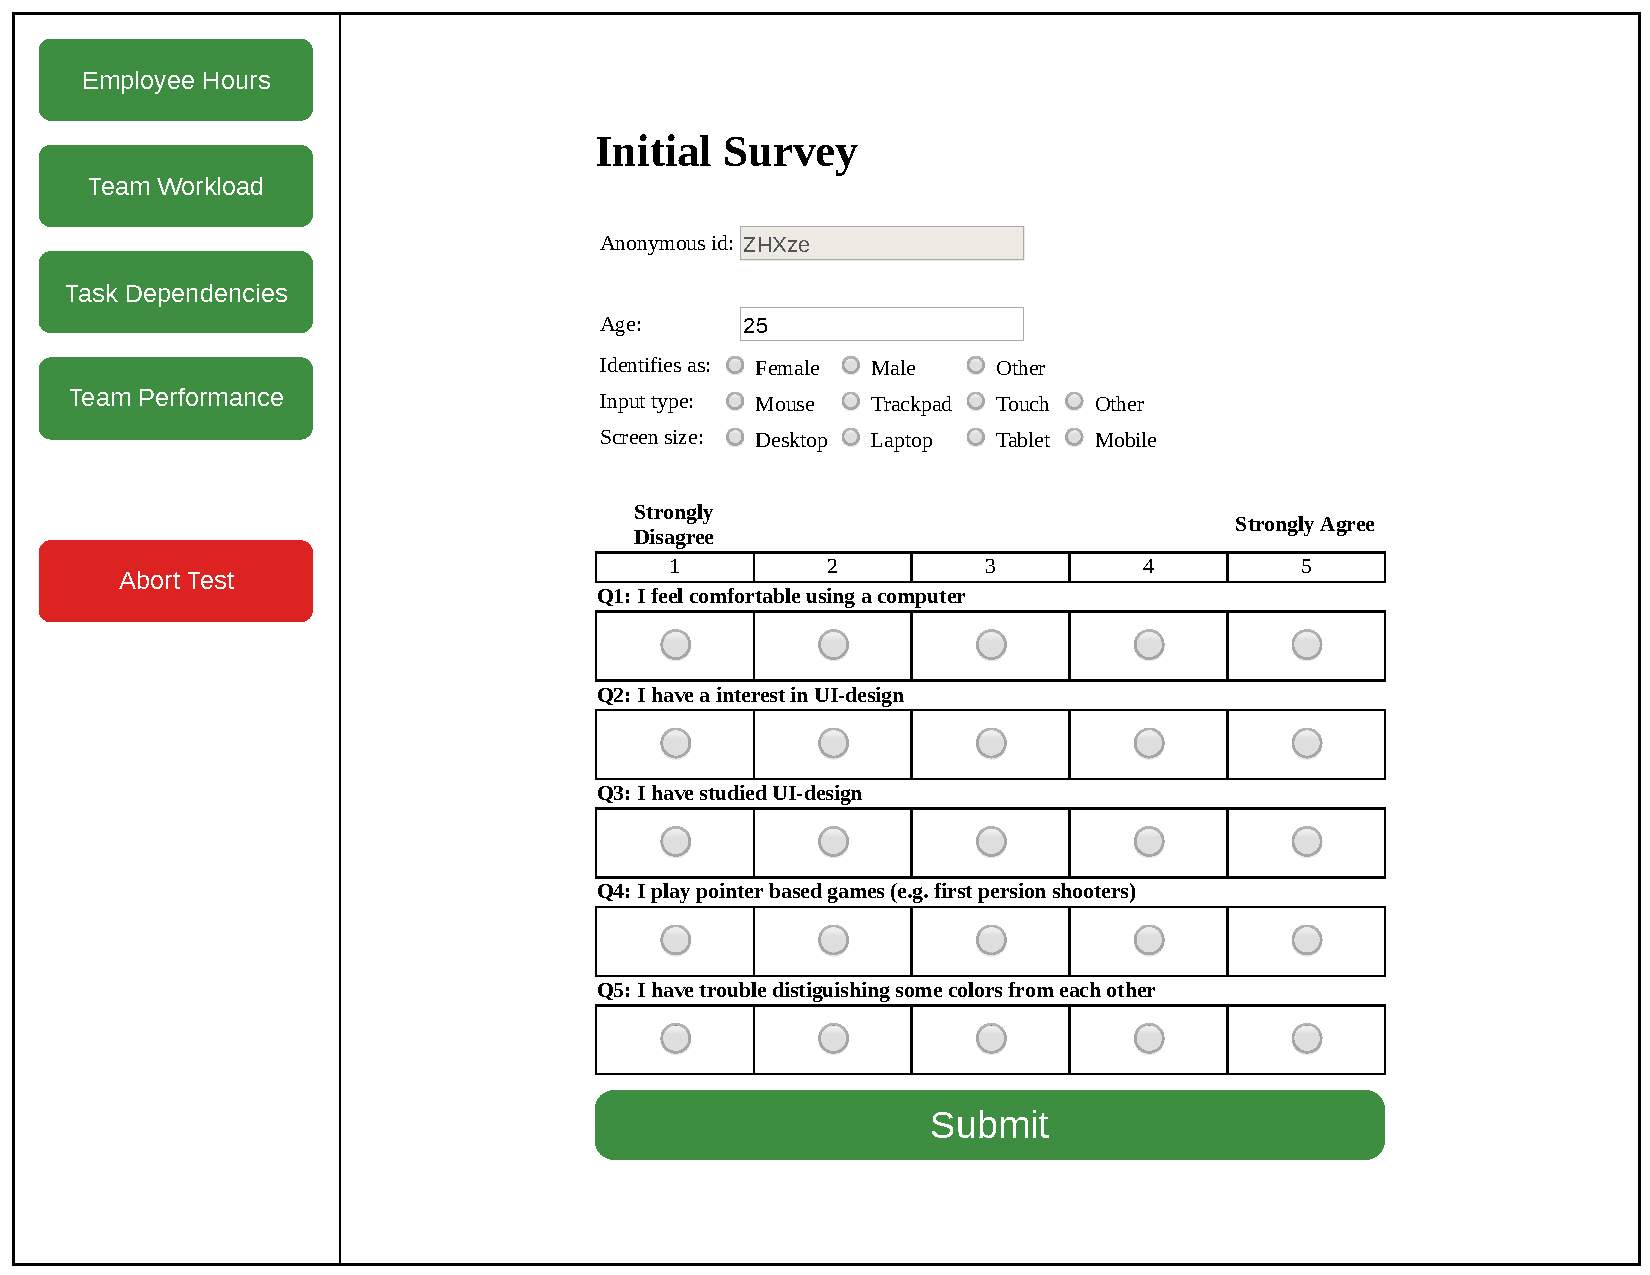
\includegraphics[width=.65\textwidth]{figures/captures/webapp_pre_survey.pdf}
    \caption{Capture of initial survey page.}
    \label{label_preSurvey}
  \end{figure}

  While it is possible for the participant to interact with the buttons on
  the left side before the initial survey is submitted, pressing any of the
  buttons except 'Abort Test' will only display the same survey-page.

  \begin{figure}[h!]
    \centering
    \fbox{
      \includegraphics[trim={4cm 8cm 9cm 8cm},clip,width=.5\textwidth]{figures/captures/webapp_abort.pdf}
    }
    \caption{Capture of confirmation page for aborting the test.}
    \label{label_abort}
  \end{figure}

  The dedicated 'Abort Test' button is available in all the different
  views of the application, in case the participant no longer wants to
  participate for any reason. Pressing this button displays a page
  explaining that continuing will scrub any activity related to their
  current anonymous id from the database and abort the current test.
  %Additionally and return it to the pool
  %of available identification strings.

  While the choices for the input method, except the last one, corresponds
  directly to a concrete input method used in human-computer interactions, the
  screen-sizes are somewhat ambiguous. This was an active choice in order to
  not alienate participants by forcing them to specify an actual measurement
  for the screen size. The assumed values for the screen-sizes ranges for the
  given choices are:
  \textit{Desktop} $>$17",
  \textit{Laptop}  12"-17",
  \textit{Tablet}  7"-12" and
  \textit{Mobile}  $<$7".

  \subsection{Landing page}

  After the participant has submitted the pre-survey, it  disappears and is
  replaced by a few basic statistics about the current test session.
  The functionality of the left-side buttons is restored and makes it
  possible to choose any of the following four test types:
  \textit{Employee Hours},
  \textit{Team Workload},
  \textit{Task Dependencies} and
  \textit{Team Performance}.

  \begin{figure}[h!]
    \centering
    \includegraphics[width=.7\textwidth]{figures/captures/webapp_main_statistics.pdf}
    \caption{Capture of the hub page, post initial survey, default state.}
    \label{label_mainStatistics}
  \end{figure}

  The session-statistics include the participants assigned anonymous id,
  how many test of each type they have completed and how many test they
  have to complete in order for the post-survey to become available.

  As previously stated, requiring five tests before making the post-survey
  available is the only hard limitation placed on the participants. Other than
  the test-minimum there is no limit on how many tests they can perform or how
  long time they take to complete a individual test or the test session as a
  whole.

  \subsection{Information, fictional context and execution}

  Before starting any of the tasks, the participant is greeted by a page
  containing the general information about the task at hand. Each of the pages
  follows the same general structure, three sections, in the following order
  \textit{Goal}, \textit{How} and \textit{Summary}.

  According to the guidelines for on-screen
  text\cite{citeOptimalLineLengthinReadingALiteratureReview}, a line should be
  around 55 characters long in order to maximize the ease of reading and
  comprehension. Any line shorter than 25 character or longer than 100
  character is detrimental to the reading experience.

  Keeping this in mind, the goal sections should be a short summary that
  informs the participant what they need to do in order to complete the task
  successfully.

  After reading the how section, the participant should have a
  basic understanding of how the information related to the test is
  structured and presented. If there are any specific details about the
  representation of the task that are deemed essential they should be
  described in this section.

  Finally, the summary section is meant to repeat the information in the how
  section, but in a different and briefer fashion in an attempt to help with
  user retention.

  Lastly, the participant is told that the same information that has just
  been presented is available after starting the test, accessible by
  hovering the cursor over a '?' in the upper left corner.

  Since all the task-mechanics boil down to
  \textit{find the element and press it as fast as possible},
  the intent is to give the participant enough concrete
  information about the test at hand while trying to maintain the
  implied fictional context of the task. Which means the tone of any
  instructions or information should be closer to
  \textit{''select the co-worker with the most X''} rather than
  \textit{''click the largest box''}.

  \subsection{Employee hours}

    \textit{\ideaOne}

    The premise for this task is that the organization generating the data
    utilizes some form of task assigning system together with a
    cost-estimation system. In short, there is a set of tasks that need to
    be done, each with a estimated time-cost, and a number of people that
    can be scheduled to do said work.

    Given there is a limited amount of time that any assignee can spend
    working, it is possible to over-schedule someone. In this scenario,
    being over-scheduled is the result of having more work scheduled to you
    over a period of time than the total available capacity for the same
    period. In summary, the goal of this task consists of identifying these
    cases, in particular, the person that is the most over-scheduled.

    \begin{figure}[h!]
      \centering
      \includegraphics[width=.49\textwidth]{figures/captures/webapp_employee_hours_info.pdf}
      \includegraphics[width=.49\textwidth]{figures/captures/webapp_employee_hours_task.pdf}
      \caption{Capture of Employee Hours information and task page.}
    \end{figure}

    After starting the task, the participant is shown a bar-graph with bars
    of varying heights and coloring. Each bar shows the relation between
    available and scheduled work-time for one out of the twenty-five
    represented people.

    Here, the height of the black outline of each bar represents the
    \textit{available work-capacity}, the varying heights simulating the
    difference of available hours due to to sick-leave, vacations or
    different contracts.

    The \textit{total scheduled workload} for
    each person is represented by the height of the colored segments in
    each bar. If there is capacity left the colored segment will not extend to the
    top of the bar outline, leaving a white segment representing
    non-scheduled time. On the other hand, if the amount of scheduled work
    is greater than the available capacity, the color will extend beyond
    the original outline and be colored differently for readability.

    In summary, the height of a white segments in a bar represent the
    amount of remaining capacity, while the height of any other-colored
    segment signifies how \textit{over-scheduled} someone is. Find the
    largest other-colored segment it and click on it.

%      \subsection{Task - team workload}
  \newpage
  \subsection{Team workload}

    \textit{\ideaTwo}

    In the following scenario the business or organization has a schedule,
    Monday to Friday, that stretches twenty-five weeks into the future. The
    goal is to keep the workload as steady as possible without to many
    jumps in either direction. Have to little to do and people are
    underutilized and in worst case, bored. Have to much that needs to be
    done at the same time and people might burn out. Avoiding both
    extremes would be preferable.

    \begin{figure}[h!]
      \centering
      \includegraphics[width=.49\textwidth]{figures/captures/webapp_team_workload_info.pdf}
      \includegraphics[width=.49\textwidth]{figures/captures/webapp_team_workload_task.pdf}
      \caption{Capture of Team Workload information and task page.}
    \end{figure}

    Running this test shows the participant a grid of twenty-five rows
    consisting of five columns each, denoted
    \texttt{MON},
    \texttt{TUE},
    \texttt{WED},
    \texttt{THU} and
    \texttt{FRI},
    representing the scheduled twenty-five workweeks mentioned above. Each
    of the rectangles are colored with the same color but differ in the
    saturation. A cell that has zero saturation, or white in this case,
    signal that no work is scheduled for completion on that particular day.
    Inversely, the darker a cell is, the more work needs to be completed on
    that specific day.

    Since there needs to be a clearly defined goal for each test, there has
    to be a choice between bored and burned out people, where the latter
    seems far worse. Now the problem can be corrected by identifying days
    where there is an extra high amount of work that needs to be done, and
    try to re-schedule it to less busy days.

    For the participant executing the test, the goal is to find the
    darkest, or most saturated rectangle and click it as fast as possible.

  \newpage
  \subsection{Task dependencies}

    \textit{\ideaThree}

    The assumption for this test is that the underlying system producing
    the data has tasks that need to be completed first in order for other
    tasks to complete in turn, in short, dependencies. This test revolves
    around answering the question
    \textit{''which elements are the most crucial for the overall
      process?''}. The answer to this question can be very useful, as an
    example, when being forced to cut back on things due to limited
    resources while trying to affect as few other things as possible.

    \begin{figure}[h!]
      \centering
      \includegraphics[width=.49\textwidth]{figures/captures/webapp_dependencies_info.pdf}
      \includegraphics[width=.49\textwidth]{figures/captures/webapp_dependencies_task.pdf}
      \caption{Capture of Task Dependencies info- and task-page.}
    \end{figure}

    Initializing this test shows the participant seventeen small circles,
    representing tasks, arranged in a larger circle. Additionally, there are
    colored lines connecting some circles together, indicating there is
    a dependency between them, more lines equals more dependencies.

    Since the stated interest in knowing how dependent the different
    moving parts are on each other, knowing which task has the most
    dependencies is a good start. In terms of what the participant has to
    do to finish the test, this translates to; find the task with the most
    connections and click on it as fast as possible.

   % \subsection{Task - team performance}
    \newpage
    \subsection{Team performance}

    \textit{\ideaFour}

    Given a working-environment where things are done in parallell it
    becomes interesting to know if a specific group or individual is
    especially effective in a certain area. Having this information makes
    it possible to assign people, if they excel at a specific area, to
    tasks that match their abilities.

    In this test there are five different task-categories,
    \textit{tickets},
    \textit{rnd},
    \textit{support},
    \textit{features} and
    \textit{maintentance}.

    \begin{figure}[h!]
      \centering
      \includegraphics[width=.49\textwidth]{figures/captures/webapp_team_performance_info.pdf}
      \includegraphics[width=.49\textwidth]{figures/captures/webapp_team_performance_task.pdf}
      \caption{Capture of Team Performance info- and task-page.}
    \end{figure}

    This task presents the participant with bars showcasing the total
    completed work-load for nine different teams over an unspecified amount
    of time.

    There are two types of information shown, the total amount of work done
    by each team, represented by the total horizontal length of the bar.
    And the amount of the total work that went into a specific
    task-section, represented by the length of each individual sub-section
    of the overall bar.
    In order to correctly answer this test, the participant first needs to
    identify which of the bars is the longest one, and then identify which
    sub-section is the largest one, and click on that one.

  \newpage
  \subsection{Post survey}

  \todo{Även här blandar du lite mellan utvärdering av det webbaserade
  systemet för testning (om uppgifterna var tydliga tex) och själva
  utformningen av innehållet (om färgerna spelade roll). Du får i text försöka
  förtydliga denna blandning av fokus genom rapporten. }

    As the participant completes five or more tests the 'Take Survey'
    button becomes active, pressing this button sends the participant to
    the post-survey page. Other than the survey itself, there is also the
    option to return to the tests if the button was pressed by accident or
    if the participant had a change of mind.

    The post-survey consist of eight questions and an optional input field
    for additional comments. These questions are ment to evaluate the
    participants thoughts about the current iteration of the testing
    application in order to derive possible improvement for the next
    implementation iteration.

    \begin{figure}[h!]
      \centering
      \includegraphics[trim={2.0cm 4cm 2.0cm 5cm},clip,width=.7\textwidth]{figures/captures/webapp_post_survey.pdf}
      \caption{Capture of the post-survey.}
    \end{figure}


    Options that are of interest include, among others, if the goal of each
    task was clear, if the application was pleasing to look at, if the use of
    colors help when navigating application, etcetera. For a larger version of
    the capture, see figure 8.7 in the appendices.
